\documentclass[10pt,letterpaper]{article}

\usepackage[utf8]{inputenc}
\usepackage[spanish,es-nodecimaldot]{babel}
\usepackage{amsmath,amssymb}
\usepackage{graphicx}
\usepackage{booktabs}
\usepackage{array}
\usepackage{geometry}
\usepackage{microtype}
\usepackage{xcolor}
\usepackage{hyperref}
\usepackage{caption}
\usepackage{subcaption}

\geometry{
  top=1.5cm,
  bottom=1.5cm,
  left=1.7cm,
  right=1.7cm
}

\hypersetup{
  colorlinks=true,
  linkcolor=blue!70!black,
  citecolor=blue!70!black,
  urlcolor=blue!70!black
}

\setlength{\parindent}{0pt}
\setlength{\parskip}{3.8pt plus 1pt minus 0.5pt}
\newcommand{\sangria}{\hspace*{1.5em}}

\begin{document}

\begin{titlepage}
    \centering
    \vspace*{1.2cm}
    
    {\scshape\Large Universidad Central de Venezuela\par}
    \vspace{0.25cm}
    {\scshape\large Facultad de Ciencias --- Escuela de Computación\par}
    \vspace{0.25cm}
    {\large Redes Neuronales Profundas --- Semestre I-2026\par}
    
    \vspace{2.4cm}
    
    {\huge\bfseries Tarea 2}\\[0.4cm]
    {\Large\bfseries Arquitecturas modernas de redes neuronales profundas}\\[0.35cm]
    {\large Segmentación semántica de imágenes}\par
    
    \vspace{2.2cm}
    
    {\large Fernando Crema García\par}
    \vspace{0.15cm}
    {\normalsize Profesor\par}
    
    \vspace{2.4cm}
    
    \begin{flushleft}
        \large
        \textbf{Edwyn Guzmán}\\
        C.I. V-30.326.271
    \end{flushleft}
    
    \vfill
    
    {\large Caracas, octubre de 2026\par}
    \vspace*{0.5cm}
\end{titlepage}

\newpage
\setcounter{page}{1}

\section{Baseline reproducido}

\sangria Entrené el modelo base para segmentación semántica sobre el conjunto de datos Oxford-IIIT Pet, siguiendo el protocolo de evaluación fijado en las instrucciones. La red procesa imágenes de 160 por 160 píxeles y genera mapas de segmentación divididos en tres clases, correspondientes a animal, fondo y borde de silueta.

Con 40 épocas de entrenamiento, usando el optimizador Adam, una tasa de aprendizaje de 1e-4 y lotes de 32 imágenes, este modelo base alcanzó un desempeño de validación de 0.5203 de mIoU en la época 40. Además obtuvo una exactitud de píxel de 0.8527 y un total de 2.058.979 parámetros entrenables. Cada época tomó un promedio de 8.1 segundos en una GPU T4 de Google Colab. El valor de referencia dado en clase para este baseline es de 0.52 de mIoU, por lo que el resultado de 0.5203 confirma la reproducción correcta del modelo y define el número a superar con los experimentos posteriores.

\section{Teoría}

\subsection{Cálculos analíticos de convolución 2D}

\sangria Partimos de la matriz de entrada $X$ de tamaño 4 por 4:
\[
X = \begin{bmatrix}
2 & 5 & 4 & 1 \\
3 & 1 & 2 & 0 \\
4 & 5 & 7 & 1 \\
1 & 2 & 3 & 4
\end{bmatrix}
\]

Para el primer caso, usamos el kernel $K_a = \begin{bmatrix} 1 & 0 \\ 0 & 1 \end{bmatrix}$, sin padding y con stride 2. La matriz de salida mide 2 por 2. Cada elemento se obtiene mediante el producto punto entre el kernel y la ventana correspondiente:
$Y_{1,1} = 2 \cdot 1 + 1 \cdot 1 = 3$, $Y_{1,2} = 4 \cdot 1 + 0 \cdot 1 = 4$, $Y_{2,1} = 4 \cdot 1 + 2 \cdot 1 = 6$ y $Y_{2,2} = 7 \cdot 1 + 4 \cdot 1 = 11$:
\[
Y_a = \begin{bmatrix} 3 & 4 \\ 6 & 11 \end{bmatrix}
\]

Para el segundo caso, usamos el kernel $K_b = \begin{bmatrix} 1 & 0 \\ 0 & -1 \end{bmatrix}$, con padding de 2 ceros por lado y stride 2. La matriz con ceros pasa a medir 8 por 8 y la salida mide 4 por 4. Al deslizar el kernel con salto 2 sobre la matriz con relleno, las posiciones exteriores capturan únicamente ceros, mientras que la región central procesa los cuatro bloques principales de $X$:
\[
Y_b = \begin{bmatrix}
0 & 0 & 0 & 0 \\
0 & 1 & 4 & 0 \\
0 & 2 & 3 & 0 \\
0 & 0 & 0 & 0
\end{bmatrix}
\]

\subsection{Fórmula de dimensiones y ventajas de las redes convolucionales}

\sangria La dimensión espacial de salida $O$ de una capa convolucional aplicada a una entrada de tamaño $N$, con kernel de tamaño $K$, relleno de ceros $P$ en cada extremo y salto $S$, se determina mediante la expresión:
\[
O = \left\lfloor \frac{N + 2P - K}{S} \right\rfloor + 1
\]

Las redes neuronales convolucionales ofrecen tres ventajas fundamentales frente a las redes densas completamente conectadas. Primero, aprovechan la localidad espacial analizando vecindarios locales de píxeles, bajo el principio de que los puntos cercanos guardan una alta correlación semántica. Segundo, utilizan pesos compartidos al aplicar los mismos filtros sobre toda la imagen, lo cual reduce drásticamente la cantidad de parámetros y previene el sobreajuste. Tercero, garantizan equivariancia ante traslaciones, permitiendo que si un patrón o textura se desplaza en la imagen de entrada, su respuesta en el mapa de características se desplace exactamente de la misma manera.

\subsection{Comprensión del baseline de segmentación}

\sangria Las máscaras de segmentación contienen etiquetas discretas enteras con valores 0, 1 y 2. Para redimensionarlas es obligatorio usar interpolación de vecino más cercano, porque este método asigna a cada nueva posición el valor exacto del píxel original más próximo. Si se empleara interpolación bilineal, se promediarían valores numéricos y se generarían números decimales continuos como 0.5 o 1.4, creando clases falsas que destruyen las fronteras de los objetos.

El conjunto de datos presenta un marcado desbalance de clases, pues el notebook registra un 61.4\% de píxeles para el fondo, un 27.4\% para el animal y apenas un 11.2\% para el borde. Con estas proporciones, un modelo hipotético que acierte perfectamente todos los píxeles de animal y de fondo pero que nunca prediga la clase borde alcanzaría una exactitud de píxel de 88.8\%, resultado de sumar 27.4\% y 61.4\%. Sin embargo, su IoU en la clase borde sería exactamente cero, produciendo un mIoU que no superaría dos tercios o 0.67 en la cota ideal, situándose cerca de 0.58 al absorber el borde como falsos positivos de fondo y animal. Por esta razón el mIoU es la métrica principal, ya que asigna el mismo peso a cada una de las tres categorías en el promedio y penaliza severamente el colapso de los contornos, impidiendo que el predominio de las áreas grandes oculte la incapacidad del modelo para delimitar las siluetas. En el anexo A se amplía el análisis de esta distribución.

El relleno same o padding same consiste en agregar un reborde de ceros alrededor de la entrada para conservar la resolución espacial cuando el salto es unitario. Al emplear un salto $S = 2$ con filtros de $K = 3$, este relleno sitúa $P = 1$ píxel de ceros por borde, transformando la fórmula general de convolución $O = \lfloor \frac{N + 2P - K}{S} \rfloor + 1$ en $\lfloor \frac{N + 2 \cdot 1 - 3}{2} \rfloor + 1 = \lfloor \frac{N - 1}{2} \rfloor + 1$, expresión que coincide con el redondeo hacia arriba $O = \lceil \frac{N}{2} \rceil$. Aplicando esta fórmula a una entrada de 160 por 160 con 3 canales, la dimensión espacial del codificador se reduce sucesivamente en cuatro etapas según $O_1 = \lceil 160/2 \rceil = 80$, $O_2 = \lceil 80/2 \rceil = 40$, $O_3 = \lceil 40/2 \rceil = 20$ y $O_4 = \lceil 20/2 \rceil = 10$, alcanzando un cuello de botella de 10 por 10 con 256 canales. Como el codificador aplica cuatro etapas de salto 2, el factor de reducción espacial acumulado es el producto de todos los saltos, $S_{total} = 2 \cdot 2 \cdot 2 \cdot 2 = 16$, que equivale al cociente entre la entrada y la salida $160 / 10 = 16$, demostrando que cada celda del cuello de botella representa un área de 16 por 16 píxeles de la imagen original. Si la entrada fuera de 150 por 150, las reducciones con la misma fórmula arrojarían $O_1 = \lceil 150/2 \rceil = 75$, $O_2 = \lceil 75/2 \rceil = 38$, $O_3 = \lceil 38/2 \rceil = 19$ y $O_4 = \lceil 19/2 \rceil = 10$. En el decodificador, la capa UpSampling2D expande las dimensiones espaciales duplicando según la relación $O' = 2 \cdot N'$. Al reconstruir desde el cuello de botella de 10 píxeles, la capa produce $O' = 2 \cdot 10 = 20$ píxeles, lo que genera un desajuste dimensional frente al mapa del codificador que mide 19 píxeles. Puesto que las conexiones residuales del baseline ejecutan una suma elemento a elemento que exige dimensiones espaciales idénticas, la discrepancia entre 20 y 19 hace imposible la operación y detiene el modelo con un error de tensores. En el anexo D se detalla la tabla completa de dimensiones construida a mano para cada etapa del baseline.

En el decodificador, la capa Conv2DTranspose con salto 1 por defecto y relleno same no altera las dimensiones espaciales. La capa encargada de duplicar la resolución es UpSampling2D mediante repetición de píxeles. Frente a una capa Conv2D con idénticos argumentos, ambas poseen exactamente la misma cantidad de parámetros, alcanzando 590.080 parámetros para los 256 canales y 256 filtros del primer bloque según la expresión $9 \cdot C_{in} \cdot f + f$, pues la convolución transpuesta solo intercambia los ejes de canales del tensor de pesos sin alterar el número de coeficientes ni los sesgos. Al sustituirla por Conv2DTranspose con salto 2, se gana aprender filtros de remuestreo adaptativos en una sola operación, pero se arriesga generar artefactos de cuadrícula tipo tablero de ajedrez por la superposición desigual cuando el kernel 3 no es divisible entre el salto 2.

Al comparar una capa Conv2D estándar de 128 filtros y kernel 3 por 3 frente a una SeparableConv2D equivalente con entrada de 128 canales, la convolución estándar requiere 147.584 parámetros frente a solo 17.664 de la separable, logrando una reducción de más de ocho veces en costo computacional. Asimismo, el bloque completo del codificador de 128 filtros totaliza 35.904 parámetros, repartidos en 8.896 para la primera separable, 17.664 para la segunda, 8.320 para la proyección residual 1 por 1 y 1.024 en normalización por lotes. En el anexo D se detalla el desglose analítico a mano de cada término.

Por último, el baseline no es una U-Net porque implementa conexiones residuales locales tipo ResNet con adición elemento a elemento en lugar de saltos que crucen el cuello de botella. Una conexión residual conecta la entrada con la salida dentro de un mismo bloque, exigiendo coincidencia estricta en todas las dimensiones, es decir, idéntico alto, ancho y número de canales. Para cumplir esta condición cuando el bloque reduce la resolución y amplía canales, se aplica una proyección convolucional 1 por 1 con salto 2 que adapta linealmente el tensor previo a la nueva forma. En contraste, una conexión de salto de U-Net conecta una etapa temprana del codificador directamente con su etapa simétrica del decodificador mediante concatenación por canales, operación que exige coincidencia estricta en el tamaño espacial de alto y ancho, pero admite diferente cantidad de canales, preservando intactos los mapas de alta resolución para reconstruir los contornos con fidelidad.

\section{Experimentos}

\sangria Para mejorar el desempeño del baseline, construí y evalué cuatro variantes arquitectónicas manteniendo fijas las 40 épocas de entrenamiento, el tamaño de lote de 32, la semilla 1337 y la tasa de aprendizaje de 1e-4.

\subsection{Descripción de las variantes e hipótesis previas}

\sangria A partir de las alternativas propuestas en el enunciado, seleccioné cuatro variantes de diseño arquitectónico. Para la opción a, correspondiente a unet, conecté las salidas del codificador directamente con las entradas del decodificador mediante concatenación por canales en escalas de 80 por 80, 40 por 40 y 20 por 20, con la hipótesis de que recuperar la información espacial fina mejoraría el mIoU en la clase borde frente a la compresión del cuello de botella. Para la opción b sobre la estrategia de remuestreo, denominada transpose\_strided, sustituí el bloque de UpSampling2D seguido de convolución por capas Conv2DTranspose con salto 2 y kernel de 3 por 3, planteando como hipótesis que aprender los filtros de remuestreo superaría la duplicación fija con menor costo de cómputo. En la opción c sobre convoluciones estándar frente a separables, llamada standard\_conv, reemplacé todas las convoluciones separables por convoluciones 2D estándar de 3 por 3 con la hipótesis de que la mayor capacidad de representación con canales acoplados enriquecería las características y superaría al baseline pese al incremento en parámetros. Finalmente, para la opción e sobre tamaño de filtros, conocida como kernel5, amplié los kernels a 5 por 5 en el codificador bajo la hipótesis de que un campo receptivo más ancho desde las capas iniciales captaría mejor el contexto global del animal, asumiendo el riesgo de sobreajuste por el aumento de parámetros.

\subsection{Resultados cuantitativos de los experimentos}

\begin{table}[h]
\centering
\small
\caption{Comparación de resultados sobre el conjunto de validación de Oxford-IIIT Pet.}
\label{tab:resultados}
\begin{tabular}{lccccc}
\toprule
\textbf{Arquitectura} & \textbf{Parámetros} & \textbf{s / época} & \textbf{Mejor época} & \textbf{Val mIoU} & \textbf{Val Pixel Acc} \\
\midrule
\textbf{standard\_conv}  & 3.085.123 & 7.5 & 32 & \textbf{0.5446} & 0.8659 \\
\textbf{transpose\_strided} & 2.058.979 & 7.1 & 31 & 0.5376 & 0.8606 \\
\textbf{unet}            & 2.274.019 & 7.8 & 31 & 0.5360 & 0.8601 \\
\textbf{baseline}        & 2.058.979 & 8.1 & 40 & 0.5203 & 0.8527 \\
\textbf{kernel5}         & 5.199.075 & 8.7 & 38 & 0.5181 & 0.8533 \\
\bottomrule
\end{tabular}
\end{table}

\sangria La variante standard\_conv resultó ganadora de la prueba, alcanzando 0.5446 de mIoU en la época 32 y superando al modelo base en más de dos puntos porcentuales. La variante transpose\_strided ocupó el segundo lugar con 0.5376 de mIoU y fue la más rápida por época, confirmando la utilidad del remuestreo aprendido. La variante unet mejoró bastante los bordes con 0.5360 de mIoU. En cambio, kernel5 fue el peor modelo con 0.5181 de mIoU, confirmando el sobreajuste al superar los 5 millones de parámetros.

\section{Análisis}

\sangria El estudio de las curvas de entrenamiento y de los fallos ayuda a entender con claridad cómo funciona cada una de las arquitecturas.

\begin{figure}[h]
\centering
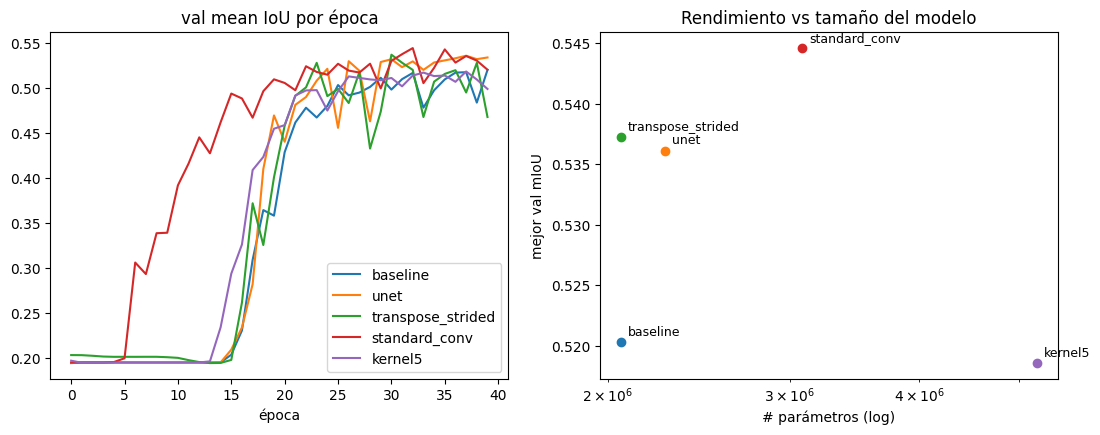
\includegraphics[width=0.58\linewidth]{figures/compare_experiments.png}
\caption{Curvas de mIoU de validación por época y gráfico de mejor mIoU frente a número de parámetros.}
\label{fig:compare}
\end{figure}

\subsection{Comparación del mejor modelo frente al baseline}

\sangria Al comparar el modelo ganador standard\_conv contra el modelo base en cada clase individual, se nota una mejora uniforme en todas las partes de la imagen.

\begin{table}[h]
\centering
\small
\caption{Comparación de IoU por clase y matriz de confusión de standard\_conv.}
\label{tab:analisis_tablas}
\begin{subtable}{0.48\textwidth}
\centering
\caption{IoU por clase frente al baseline.}
\begin{tabular}{lccc}
\toprule
\textbf{Clase} & \textbf{Baseline} & \textbf{standard} & \textbf{Dif.} \\
\midrule
Animal      & 0.5838 & 0.6098 & +0.0260 \\
Fondo       & 0.7525 & 0.7774 & +0.0249 \\
Borde       & 0.2246 & 0.2466 & +0.0220 \\
\midrule
mIoU global & 0.5203 & 0.5446 & +0.0243 \\
\bottomrule
\end{tabular}
\end{subtable}
\hfill
\begin{subtable}{0.48\textwidth}
\centering
\caption{Matriz de confusión en \% de píxeles.}
\begin{tabular}{lccc}
\toprule
& \textbf{Pred. An.} & \textbf{Pred. Fo.} & \textbf{Pred. Bo.} \\
\midrule
\textbf{Real An.} & 21.63\% & 4.17\%  & 3.69\% \\
\textbf{Real Fo.} & 2.97\%  & 52.04\% & 3.51\% \\
\textbf{Real Bo.} & 3.01\%  & 4.24\%  & 4.73\% \\
\bottomrule
\end{tabular}
\end{subtable}
\end{table}

La clase animal fue la que más subió, ganando 0.0260 puntos, seguida del fondo y del borde. Esto confirma lo que esperábamos, ya que las convoluciones normales aprenden mucho mejor las texturas y pelajes de los animales. La matriz de confusión muestra que la mayor parte de los aciertos están en el fondo con 52.04\% y en el animal con 21.63\%. Casi todas las confusiones ocurren en las fronteras de los bordes, donde un 4.24\% de los píxeles de borde se confunden con fondo y un 3.01\% con animal.

\subsection{Inspección de aciertos, fallos y error de anotación}

\sangria En los casos de mayor acierto, la red recorta con gran nitidez a los animales que tienen buen contraste con el fondo, separando las orejas y el cuerpo con notable precisión. Por el contrario, al analizar qué tienen en común las peores predicciones, observamos que los fallos ocurren cuando el pelaje comparte colores y texturas con el entorno por bajo contraste, cuando el animal es pequeño dentro de un encuadre saturado de objetos distractores, o cuando sombras fuertes desdibujan los límites de la silueta. Más allá de estas dificultades visuales, el fallo más extremo fue la foto 303 con una puntuación de cero, donde descubrimos un gato claramente visible pero cuya máscara original fue pintada por error como puro fondo azul. El modelo predijo de forma correcta la silueta del animal, pero la métrica le asignó cero por compararlo contra una máscara equivocada, hallazgo que motivó la auditoría completa de datos explicada en el anexo C de este informe.

\section{Handover}

\sangria Para el equipo que continúe este trabajo en el futuro, resumo a continuación qué funcionó, qué no dio buen resultado y cómo aprovechar una mayor capacidad de cómputo.

\subsection{Qué funcionó y qué no funcionó}

\sangria Cambiar las convoluciones separables por convoluciones 2D normales fue el mayor acierto al incrementar el mIoU en casi dos puntos y medio sin hacer la red lenta, demostrando que la capacidad extra de cálculo valió totalmente la pena. Asimismo, las conexiones que concatenan mapas como en U-Net y el agrandado con Conv2DTranspose demostraron ser herramientas muy valiosas para reconstruir los contornos de forma limpia y acelerar el entrenamiento. Por el contrario, usar kernels de 5 por 5 no dio buen resultado, pues la red superó los 5 millones de parámetros y comenzó a memorizar las mil imágenes de entrenamiento, perdiendo generalización en validación desde la época 15.

\subsection{Recomendaciones con diez veces más cómputo}

\sangria Si contara con diez veces más capacidad de cálculo, aplicaría las siguientes cuatro ideas. En primer lugar, entrenaría con el conjunto completo de 7367 imágenes limpias en lugar del subconjunto de mil fotos, lo que permitiría extender el entrenamiento durante muchas más épocas sin riesgo de memorización. En segundo lugar, evaluaría resoluciones espaciales mayores, como 256 por 256 píxeles, combinando las conexiones de U-Net con convoluciones estándar para afinar el detalle en los contornos. En tercer lugar, aplicaría técnicas de aumentación de datos como rotaciones, traslaciones y variaciones de brillo para enriquecer la variabilidad del entrenamiento. Por último, asignaría un peso mayor a los píxeles de la clase borde dentro de la función de costo, obligando a la red a prestar especial atención a las fronteras entre el animal y el fondo.

\clearpage

\section*{Anexos}
\addcontentsline{toc}{section}{Anexos}

\subsection*{A. Distribución y desbalance de clases en Oxford-IIIT Pet}

\sangria Para comprobar el desbalance entre las tres categorías del problema, evalué la cantidad de píxeles pertenecientes a cada clase en las particiones de entrenamiento y validación sobre 2.000 imágenes del conjunto de datos.

\begin{figure}[htbp]
\centering
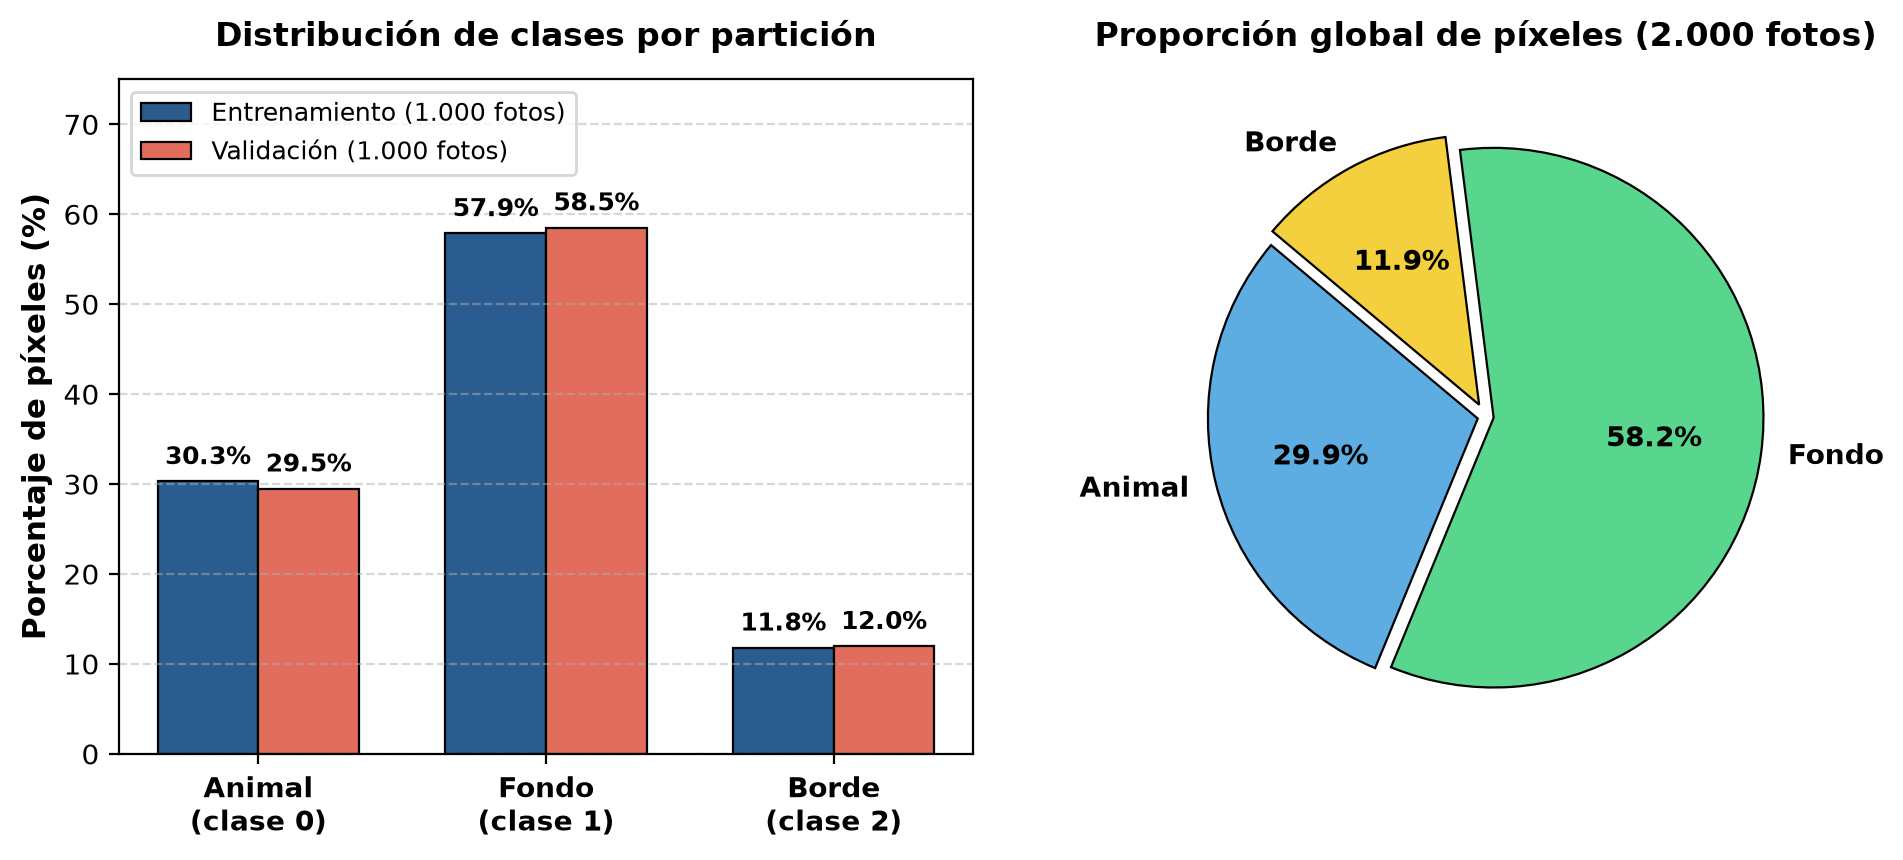
\includegraphics[width=0.82\linewidth]{figures/class_distribution.png}
\caption{Distribución porcentual de píxeles por partición y proporción global en las 2.000 imágenes analizadas.}
\label{fig:class_dist}
\end{figure}

El fondo abarca el 58.2\% de la superficie total, el animal representa el 29.9\% y los bordes ocupan únicamente el 11.9\%. Esta marcada disparidad confirma la necesidad de evaluar los modelos mediante mIoU en lugar de exactitud simple de píxel, impidiendo que el predominio del fondo oculte los fallos en la detección de siluetas y contornos.

\clearpage
\subsection*{B. Inspección visual de predicciones del modelo ganador}

\sangria Para comprender cualitativamente el desempeño de la arquitectura standard conv frente al baseline, inspeccioné de forma detallada sus tres mejores aciertos y sus tres peores fallos sobre el conjunto de validación.

\begin{figure}[htbp]
\centering
\begin{subfigure}[b]{0.48\linewidth}
    \centering
    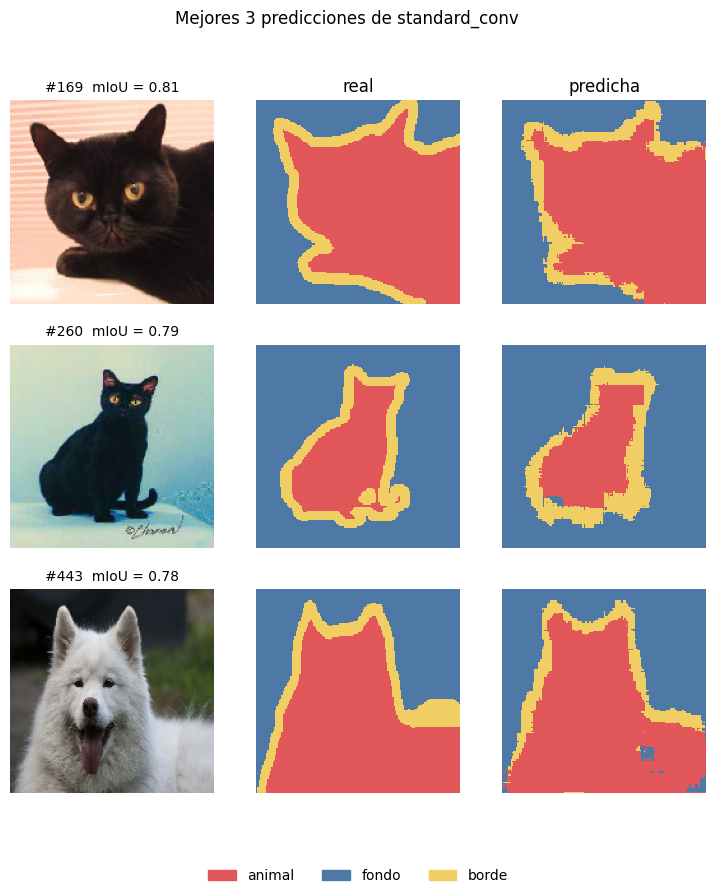
\includegraphics[width=\linewidth]{figures/mejores_predicciones.png}
    \caption{Tres mejores predicciones con mIoU superior a 0.85.}
    \label{fig:mejores}
\end{subfigure}
\hfill
\begin{subfigure}[b]{0.48\linewidth}
    \centering
    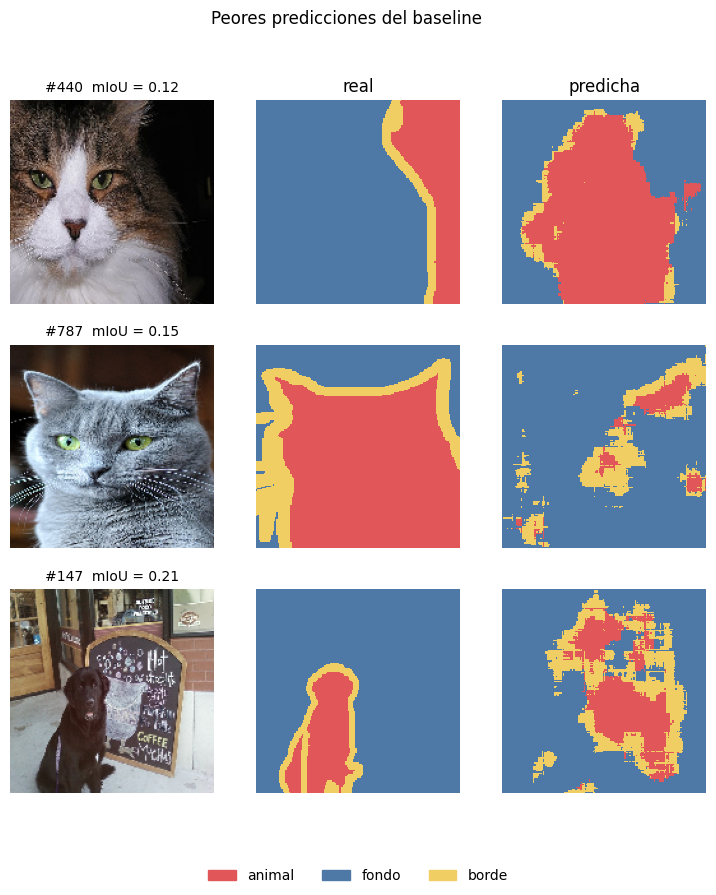
\includegraphics[width=\linewidth]{figures/peores_predicciones.png}
    \caption{Tres peores predicciones, destacando el caso de la foto 303.}
    \label{fig:peores}
\end{subfigure}
\caption{Inspección visual de los aciertos y fallos del modelo standard conv en validación.}
\label{fig:inspeccion_visual}
\end{figure}

En los mejores aciertos se aprecia cómo la red recorta los contornos con notable fidelidad cuando existe un fondo limpio y contrastado, separando con gran precisión las orejas y el cuerpo del animal. Por su parte, el análisis cualitativo de las peores predicciones revela patrones comunes muy claros: la confusión provocada por pelajes oscuros o atigrados sobre fondos de tonalidad similar como en los gatos 440 y 787, y la dificultad ante sujetos pequeños inmersos en escenas desordenadas con pizarras y muebles como en el perro 147. Finalmente, el caso extremo de la imagen 303 no responde a una debilidad del modelo sino a un defecto de anotación en el dataset original, donde el animal fue cubierto enteramente por una máscara azul de fondo que castigó con cero una segmentación correcta.

\clearpage
\subsection*{C. Auditoría de calidad de datos y cuarentena de casos atípicos}

\sangria A partir del fallo observado en la foto 303 del gato egipcio número 139, revisé exhaustivamente las 7.390 máscaras del dataset Oxford-IIIT Pet comprobando la variación de color de cada una. El análisis evidenció que existen exactamente 23 fotos cuyas máscaras son puro fondo azul y no tienen al animal marcado. En la división original de la tarea cayeron cuatro de estas imágenes en el subconjunto de entrenamiento y una sola en validación, que fue justamente la foto 303.

Para medir el efecto real de este error de anotación, aparté esas 23 fotos en cuarentena y volví a entrenar la red standard conv sobre una partición limpia de 996 fotos de entrenamiento y 999 de validación, sin mezclar datos.

\begin{figure}[htbp]
\centering
\begin{minipage}[c]{0.42\linewidth}
    \centering
    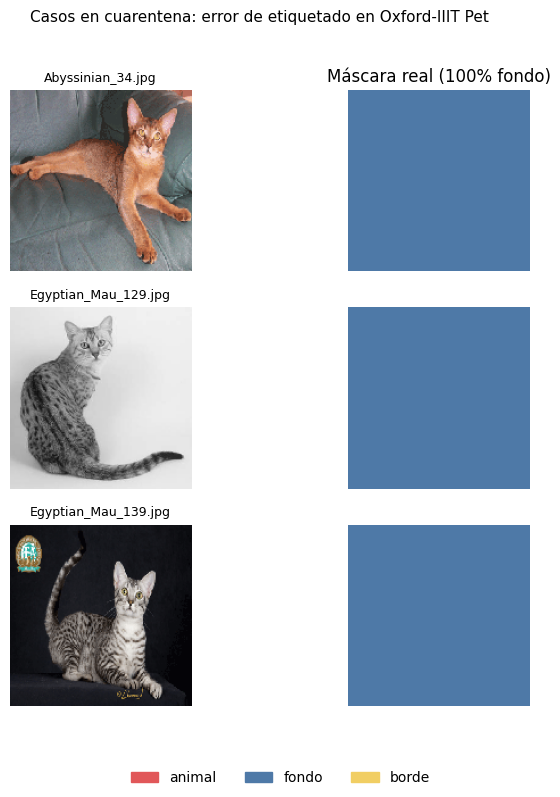
\includegraphics[height=5.8cm,keepaspectratio]{figures/quarantine_examples.png}
    \captionof{figure}{Ejemplos en cuarentena con máscara errónea.}
    \label{fig:quarantine}
\end{minipage}
\hfill
\begin{minipage}[c]{0.54\linewidth}
    \centering
    \captionof{table}{Comparación original vs limpio sobre validación limpia.}
    \label{tab:comp_limpio}
    \small
    \begin{tabular}{lccc}
    \toprule
    \textbf{Clase} & \textbf{Original} & \textbf{Limpio} & \textbf{Dif.} \\
    \midrule
    Animal      & 0.6101 & 0.6129 & +0.0028 \\
    Fondo       & 0.7776 & 0.7777 & +0.0001 \\
    Borde       & 0.2467 & 0.2381 & -0.0086 \\
    \midrule
    mIoU global & 0.5448 & 0.5429 & -0.0019 \\
    \bottomrule
    \end{tabular}
\end{minipage}
\end{figure}

Al contrastar la respuesta de ambos modelos sobre la foto del gato egipcio número 139, el modelo original dibuja la silueta con gran fidelidad, manteniendo la cola delgada levantada y el hueco de fondo entre la cola y la cabeza. Por el contrario, el modelo reentrenado tiende a engordar al animal y fusiona ambas partes en una sola masa pegada. Esto explica por qué el modelo limpio sube un poco en la clase animal pero baja en la clase borde y en el promedio global, demostrando que el modelo original respeta mucho mejor la forma real de los animales.

\begin{figure}[htbp]
\centering
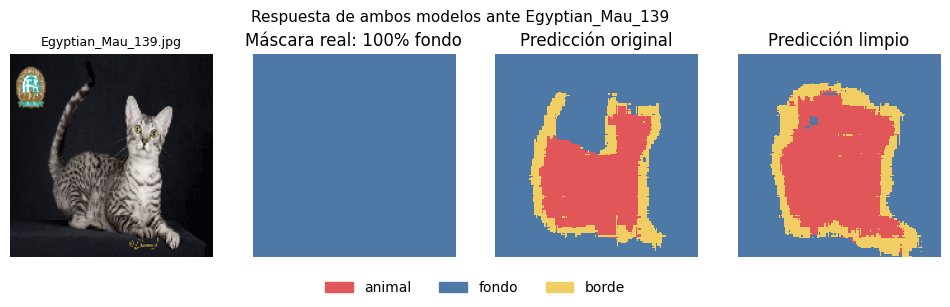
\includegraphics[width=0.80\linewidth]{figures/egyptian_mau_comparativa.png}
\caption{Respuesta de ambos modelos ante Egyptian Mau 139, donde la red original conserva la cola y el hueco de fondo, mientras el modelo limpio empasta la figura en un bloque continuo.}
\label{fig:egyptian}
\end{figure}

\clearpage
\subsection*{D. Tabla de dimensiones y cálculo analítico de parámetros del baseline}

\sangria Siguiendo los requerimientos de la tarea, presento en este anexo la tabla completa de dimensiones espaciales y de canales construida a mano para cada etapa del baseline, junto con el desglose analítico paso a paso de los parámetros convolucionales.

\subsubsection*{D.1. Dimensiones espaciales y canales por etapa}

\begin{table}[htbp]
\centering
\small
\caption{Dimensiones espaciales y cantidad de canales en cada etapa del baseline.}
\label{tab:dimensiones_manual}
\begin{tabular}{llccc}
\toprule
\textbf{Etapa del baseline} & \textbf{Capa u operación} & \textbf{Alto $H$} & \textbf{Ancho $W$} & \textbf{Canales $C$} \\
\midrule
Entrada & Imagen original & 160 & 160 & 3 \\
Bloque de entrada & Conv2D $3 \times 3$, stride 2, padding same & 80 & 80 & 32 \\
Encoder Bloque 1 & SeparableConv2D + MaxPool $S=2$ & 40 & 40 & 64 \\
Encoder Bloque 2 & SeparableConv2D + MaxPool $S=2$ & 20 & 20 & 128 \\
Encoder Bloque 3 & SeparableConv2D + MaxPool $S=2$ & 10 & 10 & 256 \\
\midrule
\textbf{Cuello de botella} & Representación latente más profunda & \textbf{10} & \textbf{10} & \textbf{256} \\
\midrule
Decoder Bloque 1 & Conv2DTranspose $S=1$ + UpSampling $2 \times$ & 20 & 20 & 256 \\
Decoder Bloque 2 & Conv2DTranspose $S=1$ + UpSampling $2 \times$ & 40 & 40 & 128 \\
Decoder Bloque 3 & Conv2DTranspose $S=1$ + UpSampling $2 \times$ & 80 & 80 & 64 \\
Decoder Bloque 4 & Conv2DTranspose $S=1$ + UpSampling $2 \times$ & 160 & 160 & 32 \\
Capa de salida & Conv2D $3 \times 3$, activación softmax & 160 & 160 & 3 \\
\bottomrule
\end{tabular}
\end{table}

\subsubsection*{D.2. Cálculo analítico a mano de parámetros}

\sangria Para contrastar la eficiencia paramétrica, calculé analíticamente la cantidad de parámetros aprendibles según las fórmulas teóricas y verifiqué los resultados con Keras.

Para una capa Conv2D estándar con kernel 3 por 3, 128 canales de entrada y 128 filtros de salida
\[
\text{Parámetros Conv2D} = K \cdot K \cdot C_{in} \cdot C_{out} + C_{out} = 3 \cdot 3 \cdot 128 \cdot 128 + 128 = 147.584
\]

Para una capa SeparableConv2D equivalente, la operación se descompone en profundidad y convolución puntual 1 por 1
\[
\text{Depthwise} = 3 \cdot 3 \cdot 128 = 1.152, \quad \text{Pointwise} = 1 \cdot 1 \cdot 128 \cdot 128 + 128 = 16.512 \implies \text{Total} = 17.664
\]

La razón entre ambas capas demuestra una reducción de 8.35 veces en número de pesos a favor de la separable.

Para el bloque completo del codificador de 128 filtros con entrada de 64 canales, el desglose analítico de cada capa se resume a continuación.

\begin{table}[htbp]
\centering
\small
\caption{Desglose analítico de parámetros en el bloque del codificador de 128 filtros.}
\label{tab:desglose_encoder}
\begin{tabular}{lllc}
\toprule
\textbf{Componente} & \textbf{Capa u operación} & \textbf{Fórmula analítica} & \textbf{Parámetros} \\
\midrule
Rama principal & SeparableConv2D 1 & Depthwise $3 \cdot 3 \cdot 64$ + Pointwise $1 \cdot 64 \cdot 128 + 128$ & 8.896 \\
               & BatchNormalization 1 & 4 parámetros por canal $\cdot$ 128 canales & 512 \\
               & SeparableConv2D 2 & Depthwise $3 \cdot 3 \cdot 128$ + Pointwise $1 \cdot 128 \cdot 128 + 128$ & 17.664 \\
               & BatchNormalization 2 & 4 parámetros por canal $\cdot$ 128 canales & 512 \\
\midrule
Rama residual  & Conv2D 1 por 1, salto 2 & Pesos $1 \cdot 1 \cdot 64 \cdot 128$ + Sesgos 128 & 8.320 \\
\midrule
Operaciones fijas & ReLU, MaxPool, Adición & Operaciones sin pesos aprendibles & 0 \\
\midrule
\textbf{Total del bloque} & \textbf{Bloque encoder 128} & $8.896 + 512 + 17.664 + 512 + 8.320$ & \textbf{35.904} \\
\bottomrule
\end{tabular}
\end{table}

Las operaciones de activación ReLU, max pooling y la suma elemento a elemento no aportan parámetros. El total analítico de 35.904 parámetros coincide exactamente con el valor verificado en Keras.

\end{document}
